% !TeX root = summary.tex
% Preamble
\documentclass[11pt]{article}
\usepackage{graphicx}
\usepackage{url}
\graphicspath{{images/}}

% Packages
\title{Introduction to Networking}
\author{Florian Lotz}
\date{2022}
% Styles:
% BOLD: \textbf{text}
% ITALIC: \textit{text}
% UNDERLINE: \underline{text}

% Document
\begin{document}
\maketitle
\tableofcontents
\pagebreak

\section{Communication Fundamentals}
    All communication methods have three elements in common\
    \begin{itemize}
    \item Sender
    \item Destination
    \item Channel
    \end{itemize}
    Rules or protocols govern all methods of communication.

    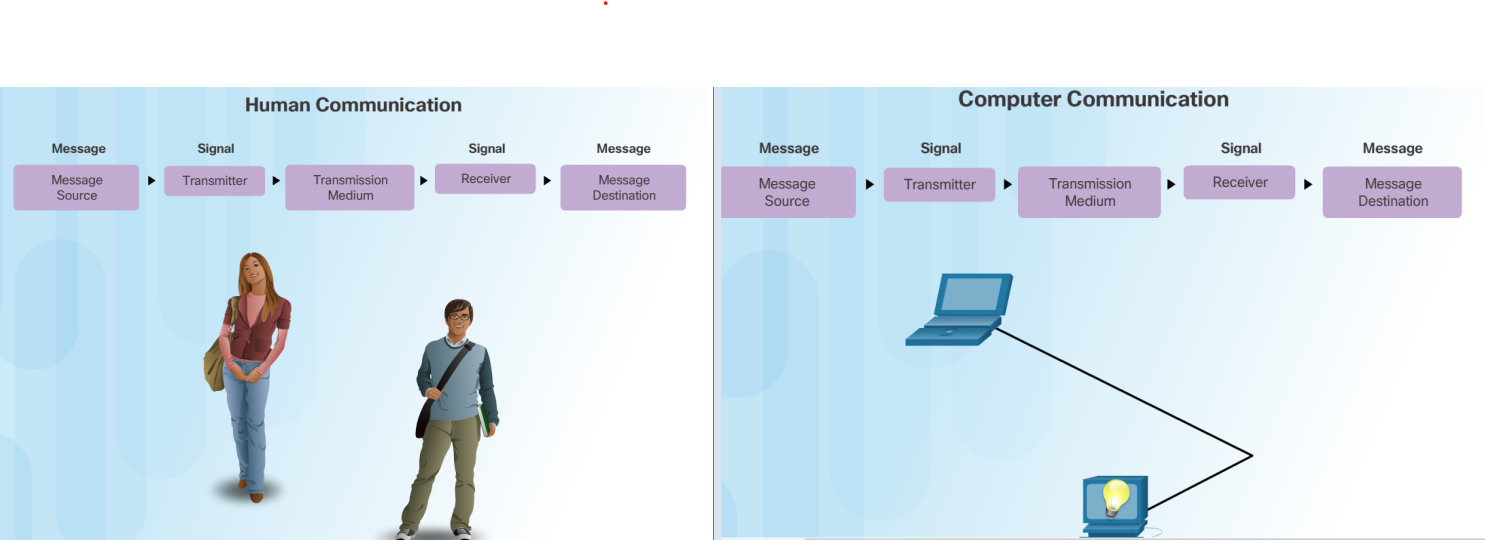
\includegraphics[width=\textwidth]{communication-fundamentals}
\subsection{Rule Establishment}
    Protocols are necessary for effective communication and include:
    \begin{itemize}
    \item An identified sender and receiver
    \item Common language and grammar
    \item Speed and timing of delivery
    \item Confirmation or acknowledgment requirements
    \end{itemize}
    Protocols used in network communications also define:
    \begin{itemize}
    \item Message Encoding
    \item Message Delivery Options
    \item Message Formatting and Encapsulation
    \item Message Timing 
    \item Message Size
    \end{itemize}
    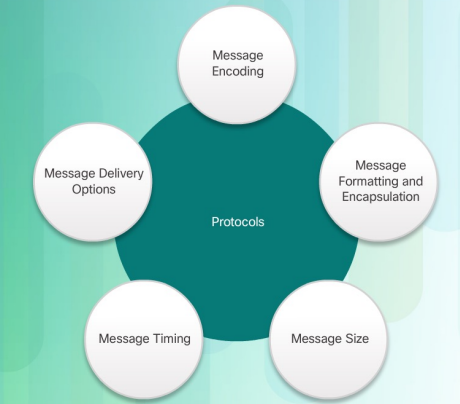
\includegraphics[width=\textwidth]{rule-establishment}
\subsection{Message Encoding}
    \begin{itemize}
        \item Encoding between hosts must be in appropriate format for the medium.
        \item Messages are first converted into bits by the sending host.
        \item Each bit is encoded into a pattern of sounds, light waves, or electrical impulses depending on the network media
        \item The destination host receives and decodes the signals in order to interpret the message.
    \end{itemize}
    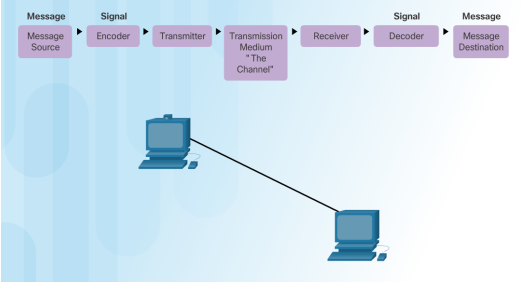
\includegraphics[width=\textwidth]{message-encoding}
\subsection{Message Formatting and Encapsulation}
    \begin{itemize}
        \item There is an agreed format for letters and addressing letters which is required for proper delivery.
        \item Putting the letter into the addressed envelope is called encapsulation.
        \item Each computer message is encapsulated in a specific format, called a frame, before it is sent over the network.
        \item A frame acts like an envelope providing destination address and source address.
    \end{itemize}
    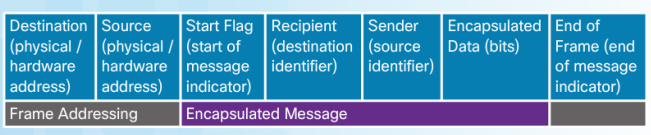
\includegraphics[width=\textwidth]{message-formatting-and-encapsulation}
\subsection{Message Size}
    Humans break long messages into smaller parts or sentences.
    Long messages must also be broken into smaller pieces to travel across a network.
    \begin{itemize}
        \item Each piece is sent in a separate frame.
        \item Each frame has its own addressing information.
        \item A receiving host will reconstruct/combine multiple frames back into the original message.
    \end{itemize}
\subsection{Message Timing}
    \begin{itemize}
        \item Access Method
        Hosts on a network need to know when to begin sending messages and how to respond when collisions occur.
        \item Flow Control
        Source and destination hosts use flow control to negotiate correct timing to avoid overwhelming the destination and ensure information is received.
        \item Response Timeout
        Hosts on the network have rules that specify how long to wait for responses and what action to take if a response timeout occurs.
    \end{itemize}
\subsection{Topology}
    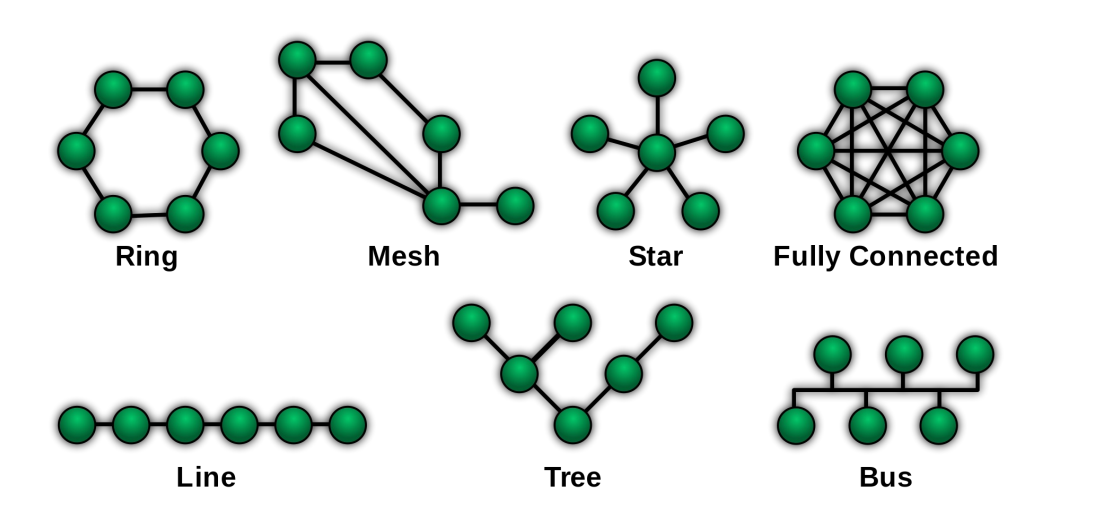
\includegraphics[width=\textwidth]{topology}
    \begin{itemize}
        \item Bus: \\
        Only one station is allowed to send data at a given time.
        Needs mechanism to avoid simultaneous sending resulting in collisions
        \item Ring: \\
        A token travels around a logical ring, regulating the channel access
        \item Star: \\
        Every station is connected to a central node
        Outage of central note implies total outage of whole topology = “Single Point of Failure”
    \end{itemize}
\subsection{(Message) Delivery Options}
    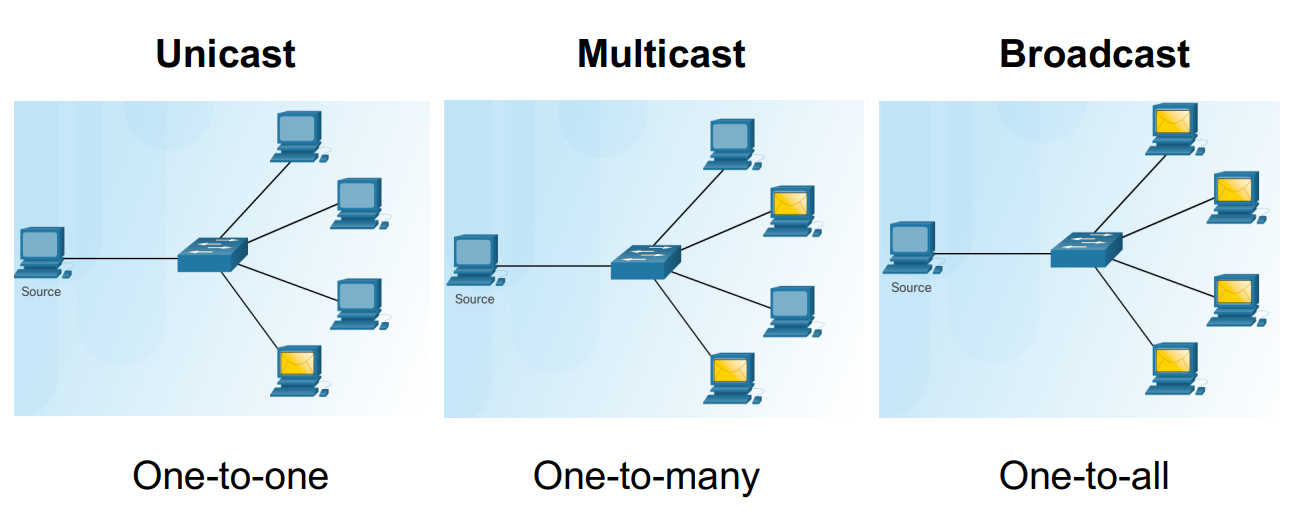
\includegraphics[width=\textwidth]{message-delivery-options}
\subsection{Method of Data Transmission}
    \subsubsection{Circuit Switching}
        One fixed line for the time of communication.
        Disadvantage: waste of bandwidth, there is just a finite number of circuits available
        
        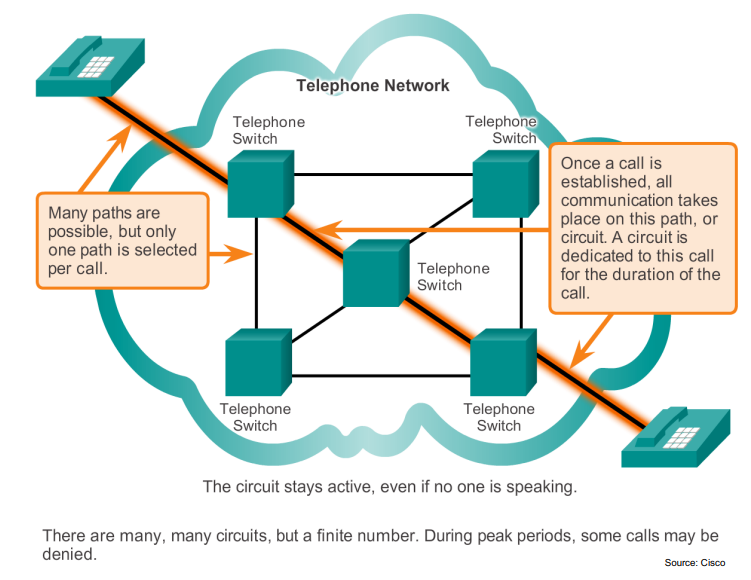
\includegraphics[width=\textwidth]{circuit-switching}
    \subsubsection{Packet Switching}
    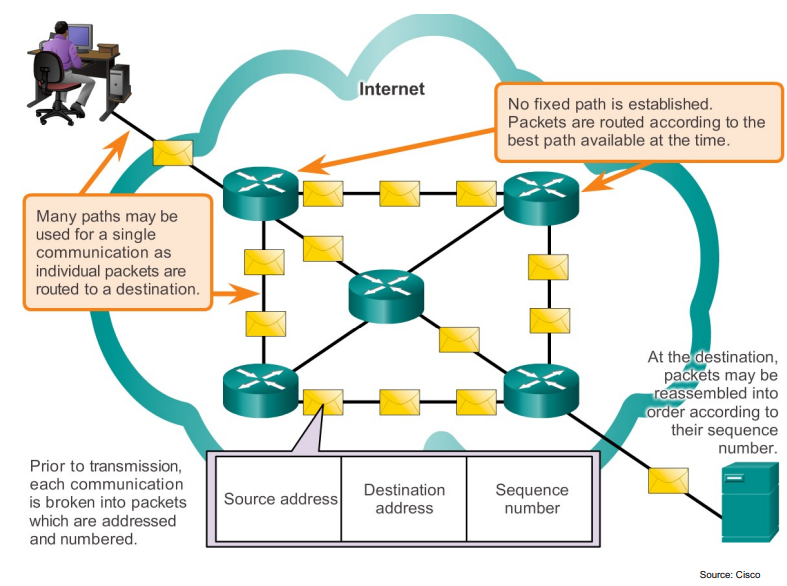
\includegraphics[width=\textwidth]{packet-switching}
    Data is split into several packets (grouped data).
    Every packet is transported through the network separately (order may change due to different paths, delays, etc.).
    Receiver needs to reassemble the packets in their original order.
    “Virtual circuits” emulate circuit switching on a packet-switched network.
\subsection{Performance}
\subsubsection{Bandwidth}
    \begin{itemize}
        \item Theoretical maximum amount of data that can be transmitted.
        \item Measuring unit: bits per second (bits/s).
        \item Bandwidth also exists in the field of signal processing à frequency range between lowest and highest obtainable frequency in Hertz.
    \end{itemize}
    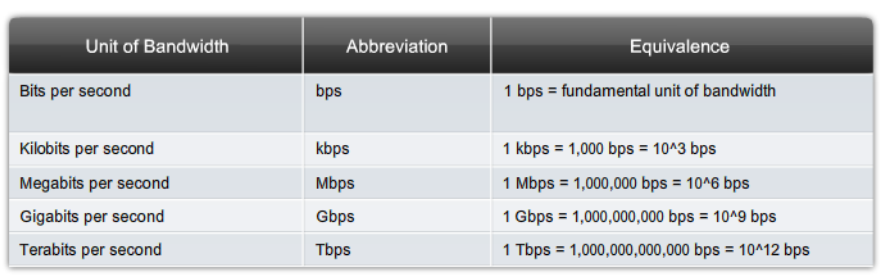
\includegraphics[width=\textwidth]{bandwidth}
\subsubsection{Latency}
    \begin{itemize}
        \item Time of transmission from one node to another
        \item Consist of different delays: the latency of the link, the queuing time, processing time in the components
        \item Round Trip Time (RTT) – amount of time from sending data until receiving the acknowledgment
    \end{itemize}
\subsubsection{Throughput}
    \begin{itemize}
        \item Amount of successful delivered data per time
        \item Depends on Bandwidth and Latency (RTT)
    \end{itemize}
\subsection{Type/Scope}
    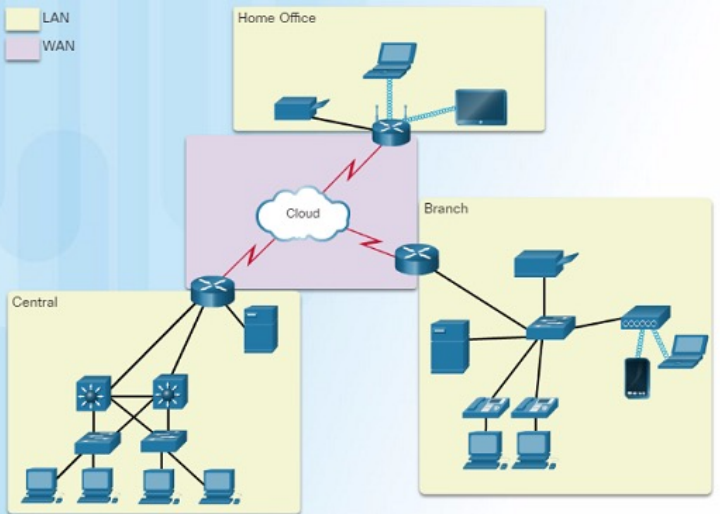
\includegraphics[width=\textwidth]{type-scope}
    \subsubsection{LAN (Local Area Network)}
    spans a small geographic area owned or operated by an individual or IT department
    \subsubsection{WAN  (Wide Area Network) }
    spans a large geographic area typically involving an Internet service provider (ISP)
    \subsubsection{Other types of networks}
    \begin{itemize}
        \item Metropolitan Area Network (MAN)
        \item Wireless LAN (WLAN)
        \item Storage Area Network (SAN)
        \item Personal Area Network (PAN), e.g.: Bluetooth
    \end{itemize}
\subsection{The Internet}
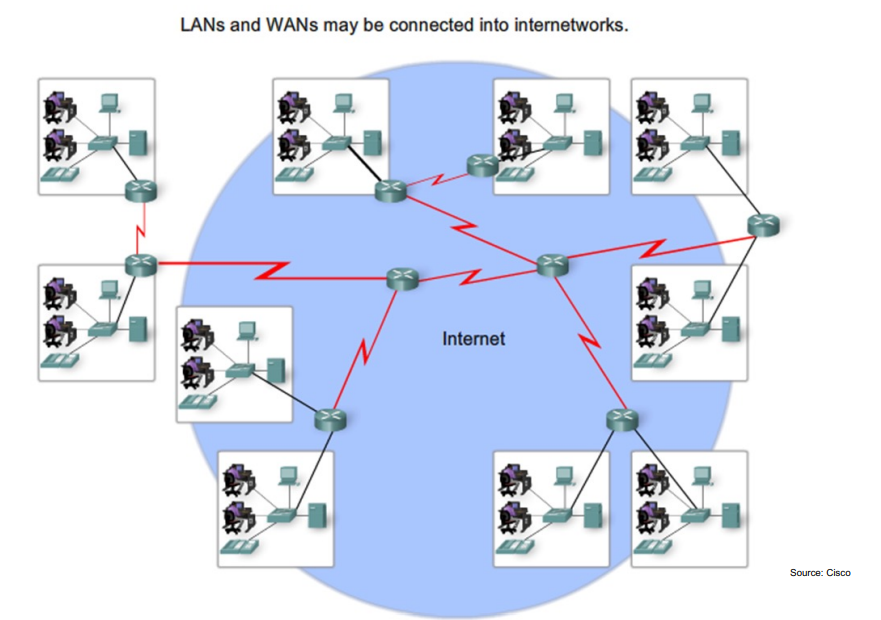
\includegraphics[width=\textwidth]{the-internet}
The purpose of the Internet is to interconnect end systems, called hosts. 
Such as PCs, servers, notebooks, smart phones, etc.
Most hosts that use the Internet are connected to a network, such as a LAN or a WAN.\@
Networks are in turn connected by routers. Each router attaches to two or more networks.
A host may send data to another host anywhere on the Internet:
    \begin{itemize}
        \item The source host breaks the data into a sequence of packets, called IP packets, or IP datagrams.
        \item Each packet includes the unique numeric addresses of the source host and destination host, called IP addresses.
        \item Based on the destination IP address, each packet travels through a series of routers and networks from source to destination.
        \item Each router, upon receiving an IP packet, makes a routing decision and forwards the packet along its way to the destination.
    \end{itemize}
    There is no “component” that is called the “Internet”
    It consists of several LANs and WANs around the world (“A Network of Networks”)
    A network on the Internet is also called Autonomous System (AS)
    \begin{itemize}
        \item An AS may consist of subnetworks
        \item Is managed by a single organization (ISP or large company)
        \item About 90,000 AS are registered by the IANA (Internet Assigned Numbers Authority)
    \end{itemize}
\subsection{How do they interconnect?}
Organizations want to interconnect their networks in a redundant manner
Different strategies:
    \begin{itemize}
        \item Transit: \\
        smaller organizations rent paths through other networks from bigger organizations
        \item Peering: \\
        Organizations make arrangements to exchange data without costs (fair use)
        \item Public Peering Points: \\
        DE – CIX Frankfurt \\
        AT – VIX Vienna 
    \end{itemize}
Biggest providers are called Tier 1 providers

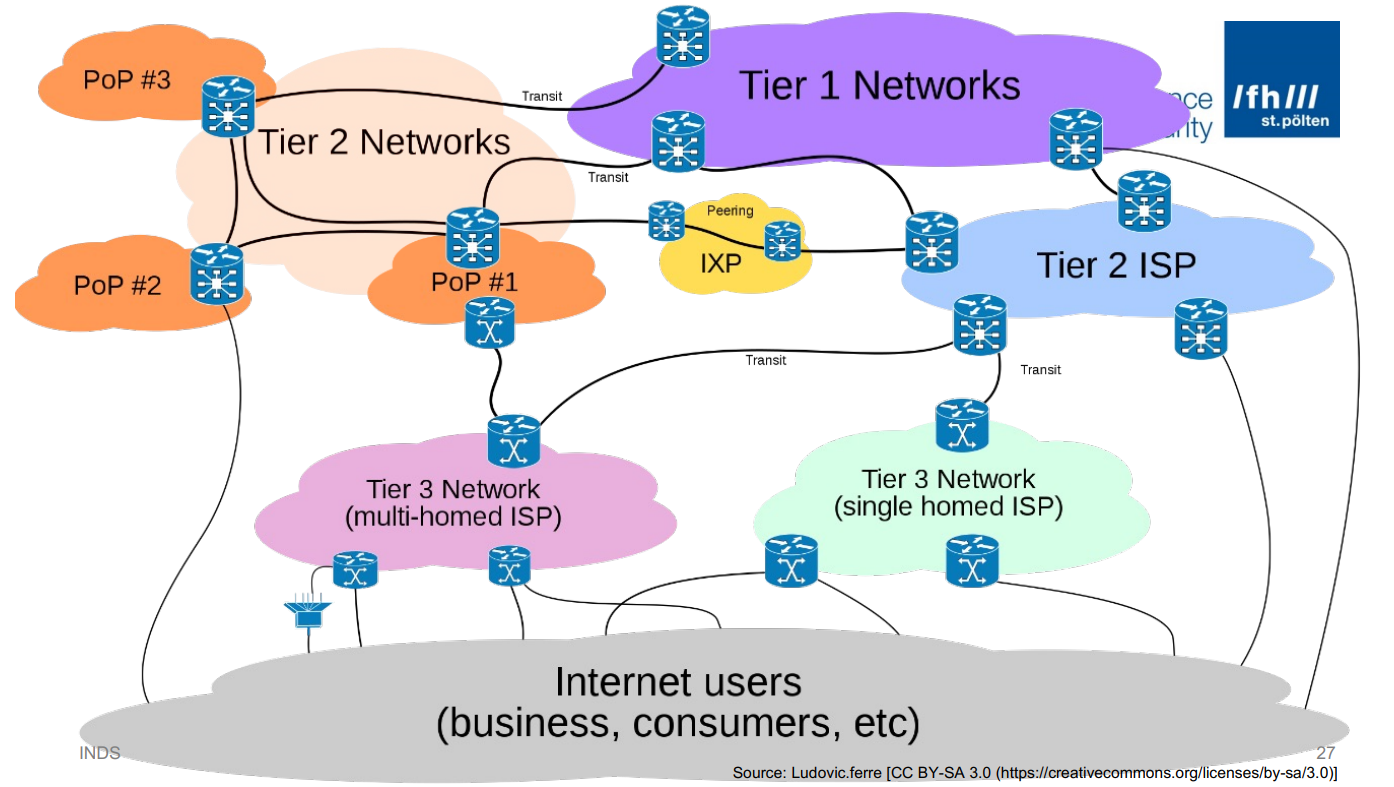
\includegraphics[width=\textwidth]{internet-interconnect}
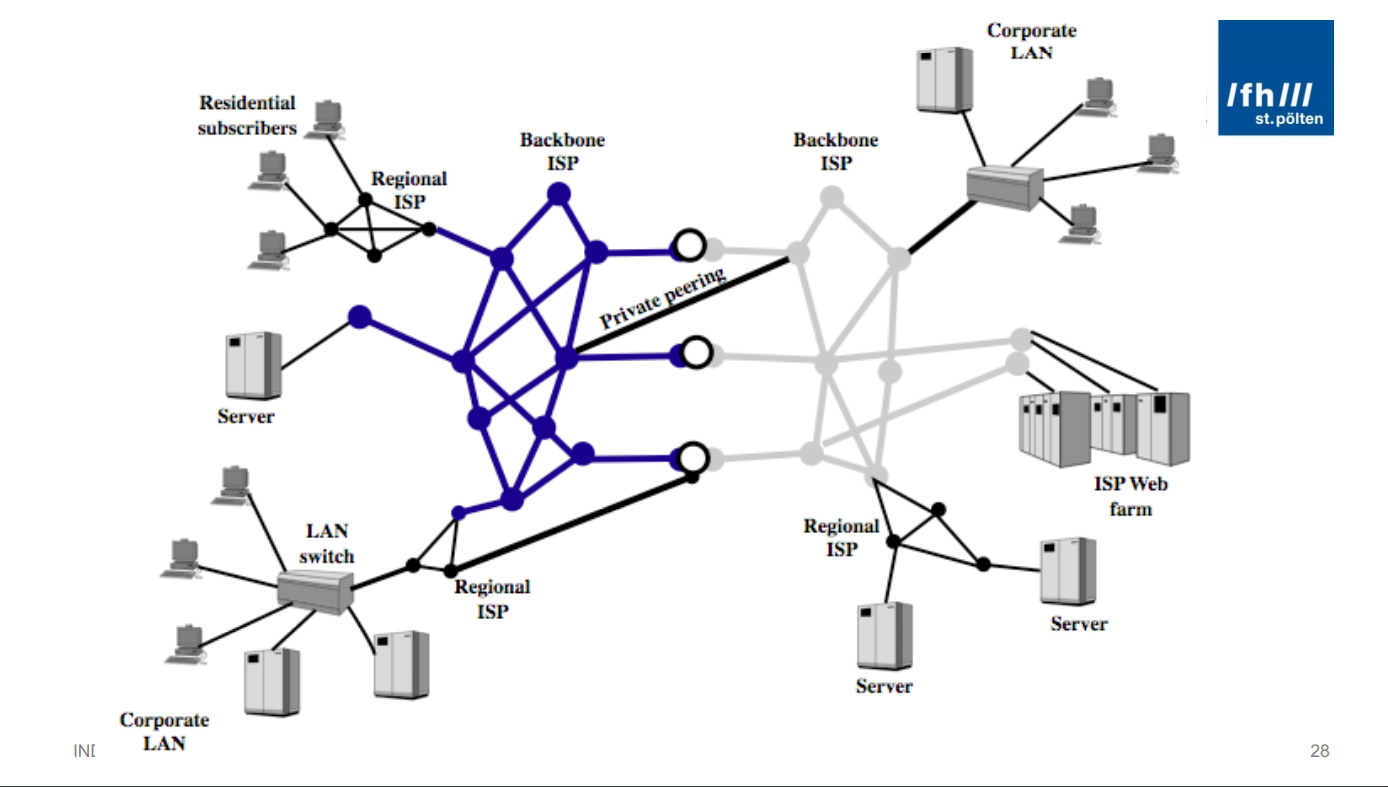
\includegraphics[width=\textwidth]{internet-interconnect-2}
\subsection{History of the Internet}
The first packet switching network and predecessor to todays Internet was the Advanced Research Projects Agency Network (ARPANET), 
which came to life in 1969 by connecting mainframe computers at four locations.
ARPANET was funded by the U.S. Department of Defense for use by universities and research laboratories. 
Bolt, Beranek and Newman (BBN) was the contractor that did much of the initial development of the ARPANET, including creating the first router known as an Interface Message Processor (IMP).
In 1973, Robert Kahn and Vinton Cerf began to work on TCP to develop the next generation of the ARPANET.\@
TCP was designed to replace ARPANETs current Network Control Program (NCP)
In 1978, TCP was divided into two protocols: TCP and IP.\@
Later, other protocols were added to the
TCP/IP suite of protocols including Telnet, FTP, DNS, and many others.
\subsection{How to connect to the Internet}
For Private Use

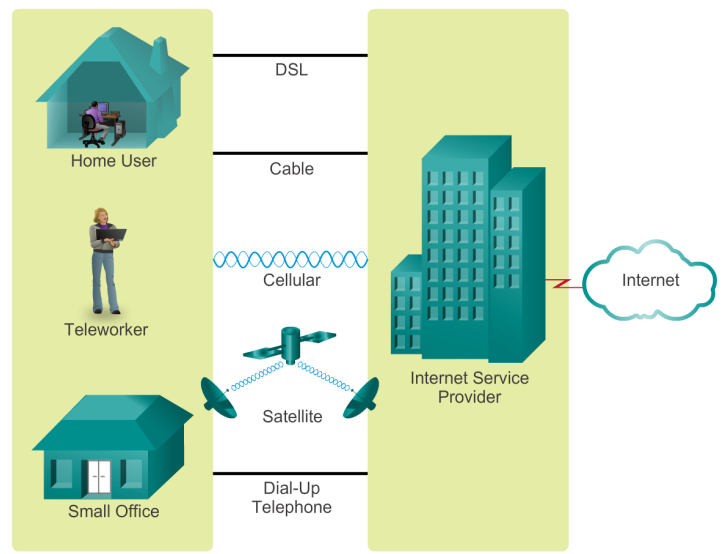
\includegraphics[width=\textwidth]{connect-internet-private-use}

For businesses

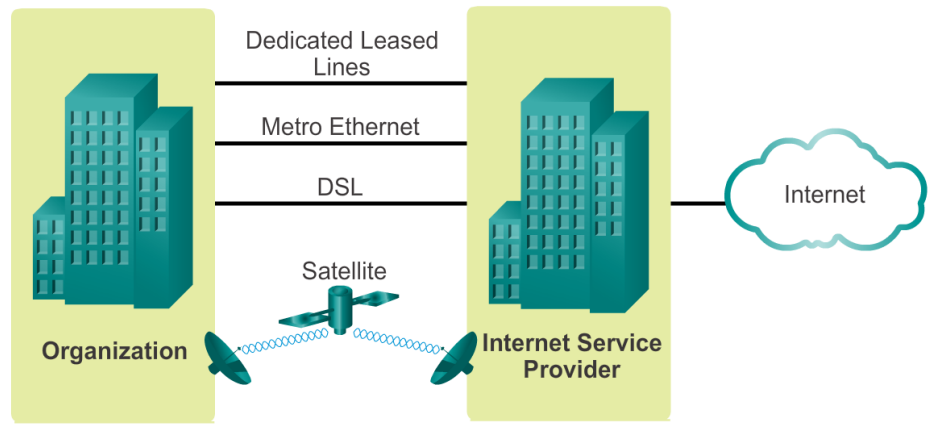
\includegraphics[width=\textwidth]{connect-internet-business-use}
\subsection{Connections between continents}
Submarine cables.
Today only fiber optical cables are used.
\@ First cable was laid in 1851 (copper cable) between France and GB.\@

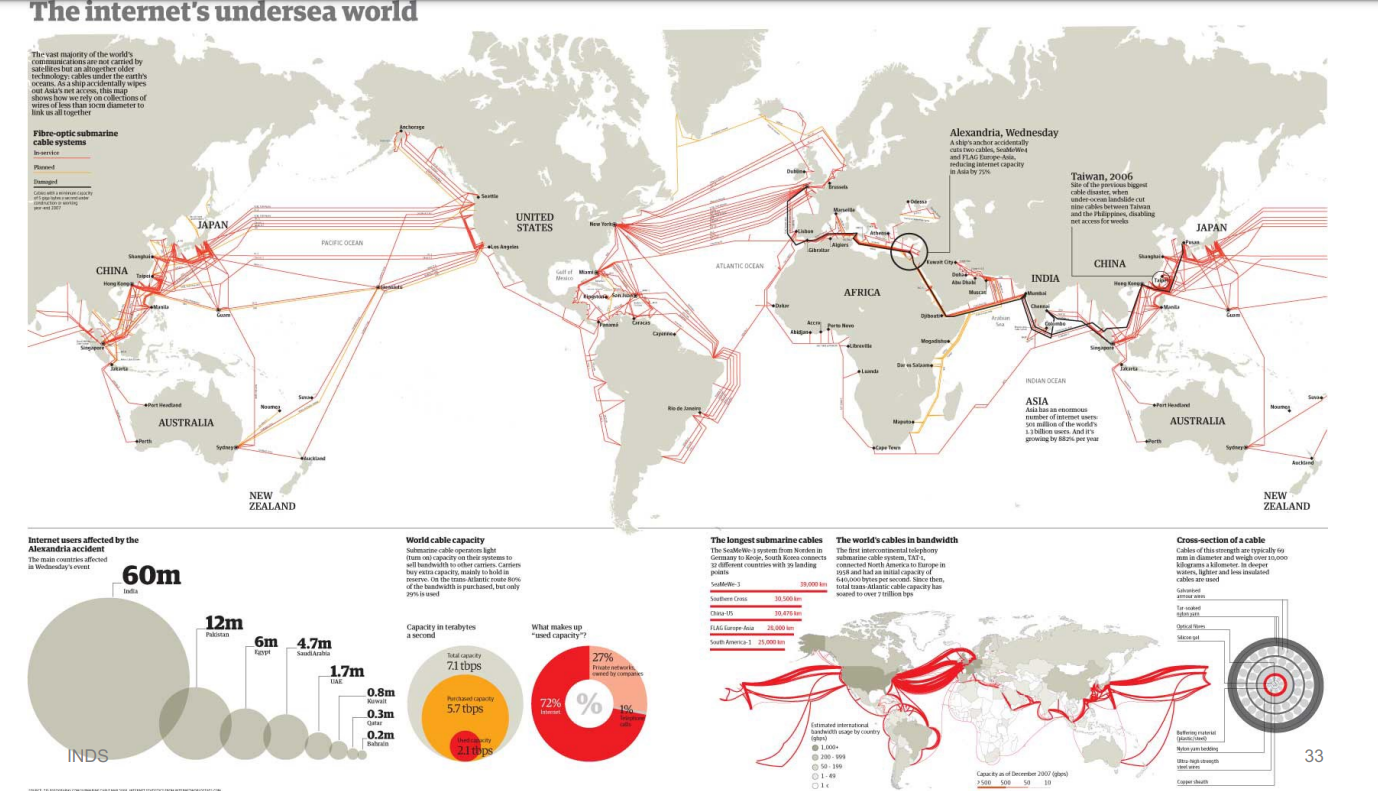
\includegraphics[width=\textwidth]{internet-connections}
\subsection{Paths through the Internet}
\url{https://traceroute-online.com/}
\subsection{Who owns the Internet?}
    \begin{itemize}
        \item Names and addresses are administered by an organization called ICANN (Internet Corporation for Assigned Names and Numbers) \\
        ICANN is a NON-profit organization
        \item IANA (Internet Assigned Numbers Authority) \\
        Department for assigning IP addresses and Names inside the ICANN
        \item The name and address spaces are split up in 5 Regional Internet Registries \\
        these distribute them to Local Internet Registries and ISPs
    \end{itemize}
\subsection{Regional Internet Registries}
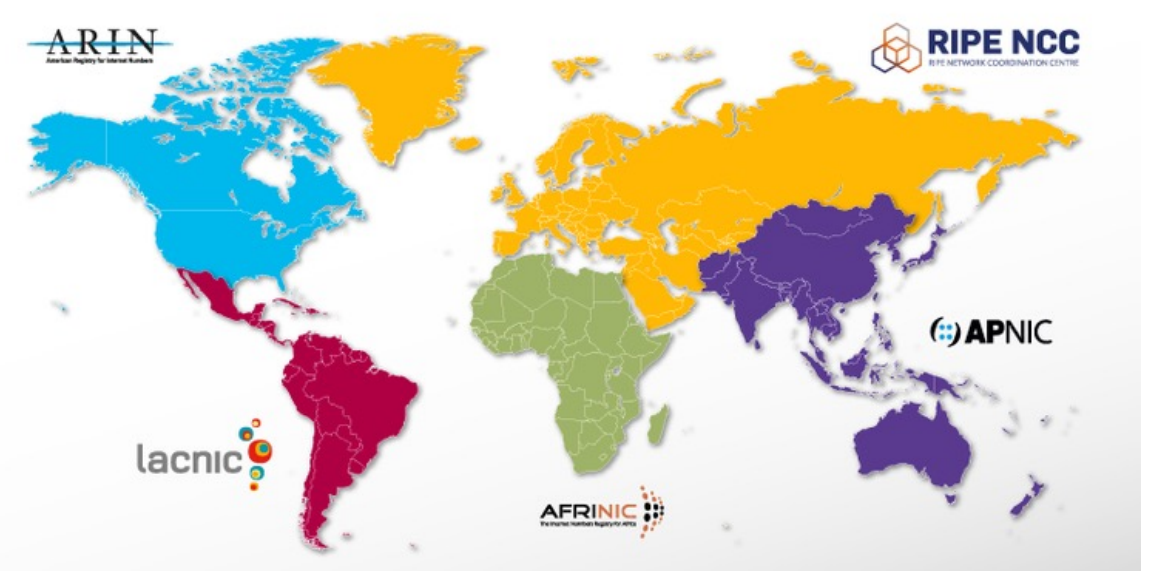
\includegraphics[width=\textwidth]{regional-internet-registries}
\section{Communication Models}
\subsection{Layered Communication Models}
    \begin{itemize}
        \item The communication task is split up in different layers with different functions – “protocol stack”
        \item Layers can only communicate with their neighbors (upper and lower) \\
        Provide “services” for each higher layer
        \item A data unit “travels” through all layers on the sender side (top-down) and then through all layers at the receiver side (bottom-up)
        \item Enhances compatibility: manufacturers have defined interfaces for each layer à following the standards allows compatible devices
    \end{itemize}
\subsection{Benefits of layered models}
\begin{itemize}
    \item Less complex: \\
    Compared to not using a layered model, network models break the concepts into smaller parts/problems.
    \item Standard interfaces \\
    The standard interface definitions between each layer allow multiple vendors to create products that fill a particular role, with all the benefits of open competition
    \item Easier to learn \\
    Humans can more easily discuss and learn about the many details of a protocol
    \item Easier to develop \\
    Reduced complexity allows easier program changes and faster product development.
    \item Multivendor interoperability \\
    Creating products to meet the same networking standards means that computers and networking gear from multiple vendors can work in the same network.
    \item Modular engineering \\
    One vendor can write software that implements higher layers, for example, a web browser, and another vendor can write software that implements the lower layers, for example, Microsoft's built-in TCP/IP software in its OSs.
specification
\end{itemize}
\subsection{OSI Model and TCP/IP Model}
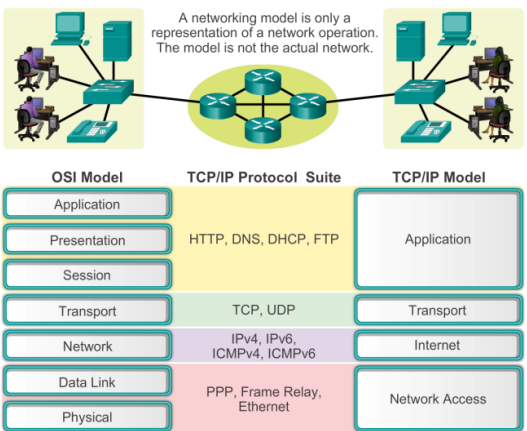
\includegraphics[width=\textwidth]{osi-and-tcp-ip-model}
\subsection{OSI Reference Model}
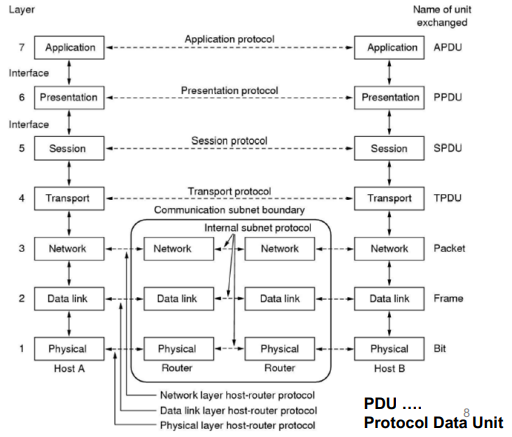
\includegraphics[width=\textwidth]{osi-reference-model}
Open Systems Interconnection (OSI) Reference Model
\begin{itemize}
    \item Standardized Model from the International Standards Organisation (ISO) 
    \item To connect open systems
    \item Consists of 7 Layers
\end{itemize}
\subsection{OSI Layer 1 – Physical Layer}
Transfer of bits over the communication channel
Tasks of the physical layer:
    \begin{itemize}
        \item Voltage level
        \item Signal duration
        \item Pinning / wire map / connectors
        \item Full Duplex / Half Duplex
        \item Transmission medium (copper, fiber, air, …)
    \end{itemize}
\subsection{OSI Layer 2 – Data Link Layer}
\begin{itemize}
    \item Logical link control Layer (LLC)
    \begin{itemize}
        \item Multiplexing for upper layer protocols (IPv4, IPv6, IPX, …)
        \item P2P Flow control (usually not used today, delegated to Layer 4 end-to-end)
    \end{itemize}
    \item Media access control layer (MAC)
    \begin{itemize}
        \item Frame delimiting and recognition
        \item Protection against errors, by generating and checking frame check sequences (FCS)
        \item Channel access mechanism on a shared medium: Carrier Sense Multiple Access (CSMA)
        \item Physical addressing (MAC addresses)
    \end{itemize}
    \item L2 Network Devices: e.g. Switches
\end{itemize}
\subsection{OSI Layer 3 – Network Layer}
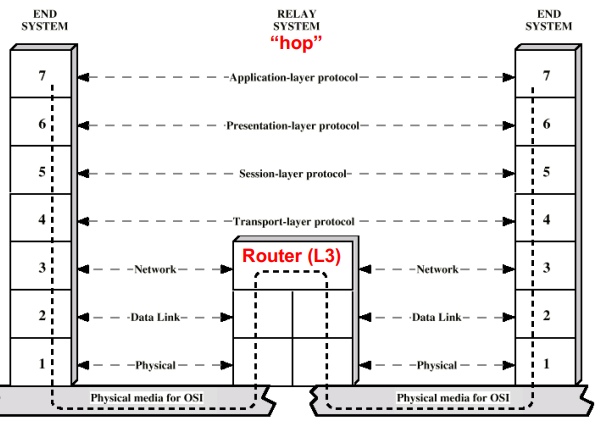
\includegraphics[width=\textwidth]{osi-3-network-layer}
\begin{itemize}
    \item Logical Addressing (e.g. IP addresses)
    \item Route selection for the packets à Chooses the best route
    \begin{itemize}
        \item Routes can be static or dynamic
        \item Routing protocols
    \end{itemize}
    \item Transmission of packets over different networks
    \item L3 Network Devices: e.g. Routers
\end{itemize}
\subsection{OSI Layer 4 – Transport Layer}
\begin{itemize}
    \item Transmits data from sender to receiver independent of the underlying network technologies.
    \begin{itemize}
        \item First End-to-End Layer
        \item Sets up a “connection” between hosts, i.e. \ end-devices / -points / -nodes
    \end{itemize}
    \item Splits the data from the session layer into smaller segments and passes them to the Network Layer
    \item Defines the kind of the service
    \begin{itemize}
        \item Connection-oriented data stream (e.g TCP)
        \item Connectionless data stream (e.g. UDP)
    \end{itemize}
    \item Connection-orientated
    \begin{itemize}
        \item Reliable
        \item Connection management (establishment, transmission, termination)
        \item Error detection
        \item Flow control
        \item Multiplexing (combining two or more data stream into one single physical connection)
    \end{itemize}
    \item Connectionless
    \begin{itemize}
        \item Not reliable
        \item Multiplexing (combining two or more data stream into one single physical connection)
    \end{itemize}
\end{itemize}
\subsection{OSI Layers 5 to 7}
\begin{itemize}
    \item Layers 5 to 7 often combined today in applications
    \item 5: Session Layer
    \begin{itemize}
        \item Provides mechanism for session management between applications
        \item Main purpose is synchronization
    \end{itemize}
    \item 6: Presentation Layer
    \begin{itemize}
        \item Defines the syntax of the transmitted data \\
        ASCII, Unicode, Jpeg, Gif, …
    \end{itemize}
    \item 7: Application Layer \\
    Defines the interface between the application (user) and the network services
\end{itemize}
\subsection{Example Devices and Protocols}
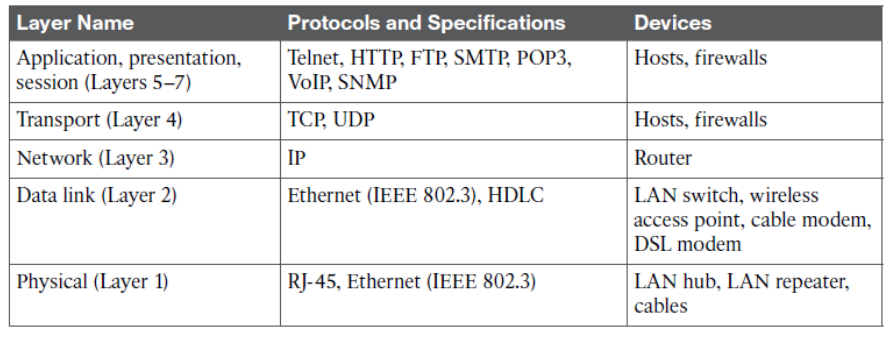
\includegraphics[width=\textwidth]{example-devices-and-protocols}
\subsection{Data transmission through the OSI Layers}
Sender wants to send data to the receiver

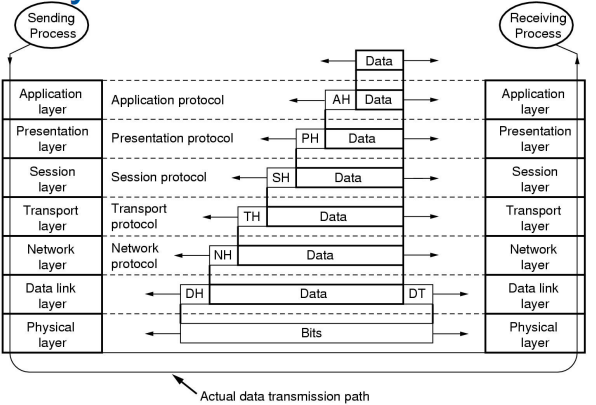
\includegraphics[width=\textwidth]{data-transmission-trhough-osi-layers}
\begin{itemize}
    \item Application Layer generates Data \\
    Passes it to the Presentation Layer and attaches a Header (AH)
    \item \ldots
    \item Network Layer \\
    Adds L3 header: e.g. \ logical addressing and several other fields
    \item Data Link Layer \\
    Adds L2 Header: e.g. \ physical addressing and attaches a checksum at end of frame
    \item Physical Layer \\
    Converts the frame to an electric signal on the wire
\end{itemize}
\subsection{Encapsulation and Segmentation}
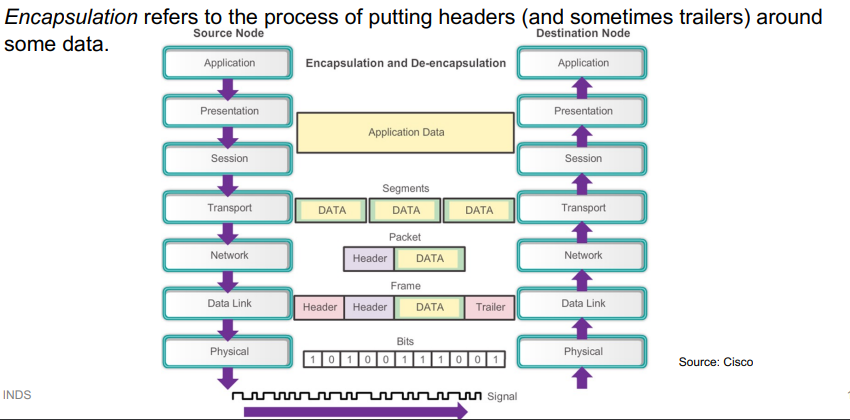
\includegraphics[width=\textwidth]{encapsulation-and-segmentation}

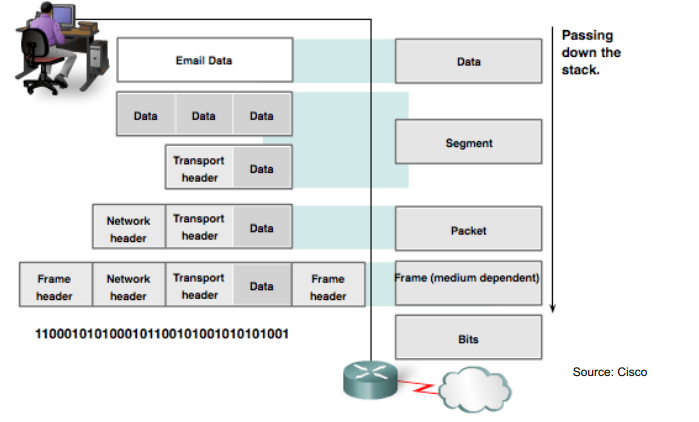
\includegraphics[width=\textwidth]{encapsulation-and-segmentation-2}
\subsection{OSI Layer – Layer Content}
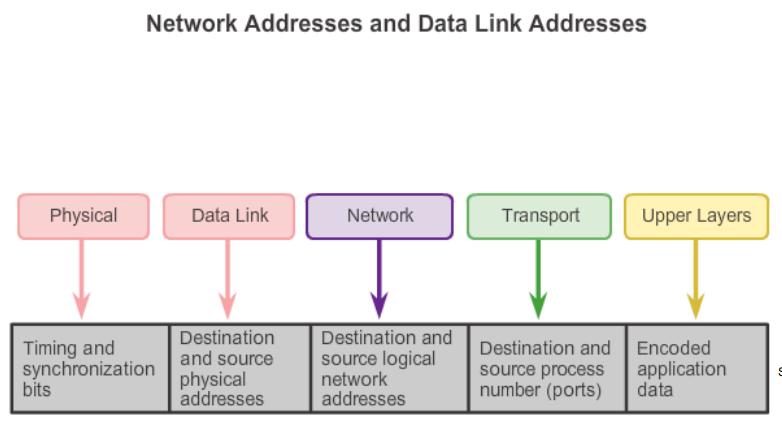
\includegraphics[width=\textwidth]{osi-layer-content}
\subsection{TCP/IP Model}
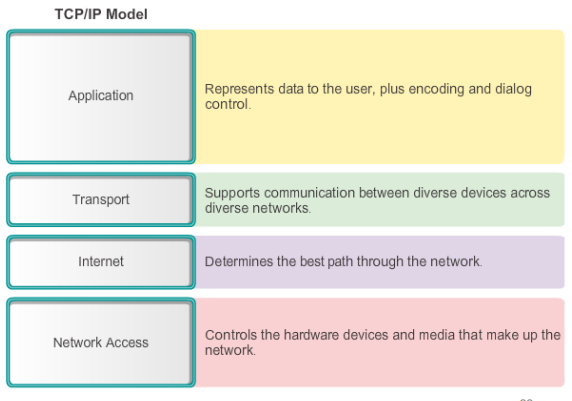
\includegraphics[width=\textwidth]{tcp-ip-model}
\begin{itemize}
    \item Network Access Layer \\
    Combines Layer 1 and Layer 2 of OSI Model (e.g. Ethernet)
    \item Internet Layer
    \begin{itemize}
        \item Transmits packets over different networks to the target
        \item Defines a packet format and a protocol: “Internet Protocol” (IP)
        \item Route selection for the packets à best path selection
    \end{itemize}
    \item Transport Layer
    \begin{itemize}
        \item TCP (Transmission Control Protocol)
        \begin{itemize}
            \item Ensures a reliable and connection-oriented data transmission
            \item Splits the data into numbered packets
            \item Acknowledges received packets
            \item Connection establishment (3 Way Handshake)
        \end{itemize}
        \item UDP (User Datagram Protocol)
        \begin{itemize}
            \item Unreliable and connectionless data transmission
            \item Use for real time applications (voice, video)
        \end{itemize}
    \end{itemize}
    \item Application Layer \\
    Consists of Layer 5 to 7 from the OSI Model
    
    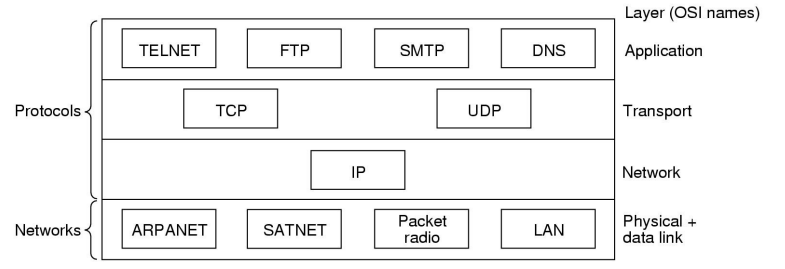
\includegraphics[width=\textwidth]{tcp-ip-application-layer}
\end{itemize}
\begin{itemize}
    \item Simplified Model
    \item Based on the ARPANET
    \item For the packet switched network
    \item Usually operating on IP (L3) and TCP or UDP (L4)
\end{itemize}
\subsection{Comparison OSI and TCP/IP Model}
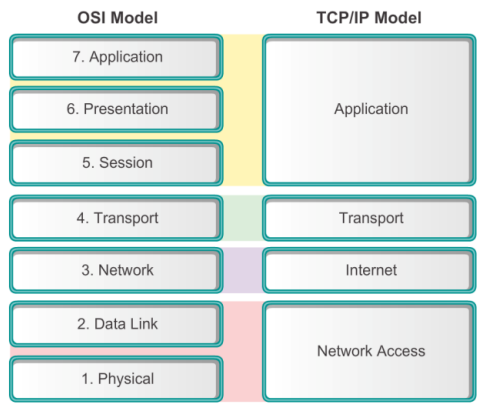
\includegraphics[width=\textwidth]{comparison-osi-tcp-ip-model}
\subsection{Standards}
\begin{itemize}
    \item Internet Society (ISOC) \\
    promotes open development and evolution of Internet use globally.
    \item Internet Architecture Board (IAB) \\
    management and development of Internet standards. 
    \item Internet Engineering Task Force (IETF) \\
    develops, updates, and maintains Internet and TCP/IP technologies.
    \item Internet Research Task Force (IRTF) \\
    focused on long-term research related to Internet and TCP/IP protocols.
    \item Internet Corporation for Assigned Names and Numbers (ICANN) \\
    coordinates IP address allocation and management of domain names.
    \item Internet Assigned Numbers Authority (IANA) \\
    manages IP address allocation, domain name management, and protocol identifiers for ICANN.\@
    \item Request for Comments (RFC) \\
    An RFC document may come from many bodies including from the Internet Engineering Task Force (IETF), the Internet Research Task Force (IRTF), the Internet Architecture Board (IAB), or from independent authors. The RFC system is supported by the Internet Society (ISOC).
    \item Institute of Electrical and Electronics Engineers (IEEE) \\
    dedicated to advancing technological innovation and creating standards in a wide area of industries including networking.
    \item Electronic Industries Alliance (EIA) \\
    standards related to electrical wiring, connectors, and network racks.
    \item Telecommunications Industry Association (TIA) \\
    standards for radio equipment, cellular towers, Voice over IP (VoIP) devices, and satellite communications
    \item International Telecommunications Union-Telecommunication Standardization Sector (ITU-T) \\
    standards for video compression, Internet Protocol Television (IPTV), and broadband communications.
\end{itemize}
\section{Physical Layer}
\subsection{General}
\subsection{(Simplified) Communications Model}
\subsection{Digital Data Transmission}
\subsection{What is the objective?}
\subsection{Terminology}
\subsection{Signals: Time Domain}
\subsection{Analogue and Digital Signals}
\subsection{Periodic Signals}
\subsection{Frequency}
\subsection{Amplitude}
\subsection{Varying Sine Waves}
\subsection{Signals: Frequency Domain}
\subsection{Addition of Frequency Components}
\subsection{Frequency Domain}
\subsection{Fourier Analysis}
\subsection{Spectrum and Bandwidth}
\subsection{Signal with DC Component}
\subsection{Data Rate and Bandwidth}
\subsection{Effective Bandwidth}
\subsection{Analog and Digital Data Transmission}
\subsection{Analog vs. Digital Data}
\subsection{Digital Signals}
\subsection{Bit Stream to Digital Signal}
\subsection{Data and Signals}
\subsection{Analog Signals Carrying Analog and Digital Data}
\subsection{Analog Transmission}
\subsection{Digital Transmission}
\subsection{Transmission Impairments}
\subsection{Attenuation}
\subsection{Attenuation Distortion}
\subsection{Delay Distortion}
\subsection{Noise}
\subsection{Channel Capacity}
\subsection{Nyquist Formula}
\subsection{Shannon Capacity Formula}
\subsection{Maximum data rate of a channel}
\subsection{Physical Layer Media}
\subsection{Transmission Media}
\subsection{Electromagnetic Spectrum}
\subsection{Guided Transmission Media}
\subsection{Copper Cable}
\subsection{Coaxial Cable}
\subsection{Coax Characteristics}
\subsection{Twisted Pair Cable}
\subsection{UTP Cable}
\subsection{Cabeling Standards}
\subsection{Transmission Methods}
\subsection{Baseband Transmission}
\subsection{Manchester Code}
\subsection{Baud Rate and Symbol Rate}
\subsection{Broadband Transmission}
\subsection{Modulation types}
\subsection{Optical Transmission (Fiber)}
\subsection{Refractive Index}
\subsection{Multi-mode Optical Fiber}
\subsection{Single-mode Optical Fiber}
\subsection{Optical Fiber Types}
\subsection{Single vs Multi-mode}
\subsection{Optical Fiber Attenuation}
\subsection{Transmitters and Receivers}
\subsection{Wavelength Division Multiplexing}
\subsection{Extending Optical Fiber Cables}
\subsection{Fiber Connectors}
\subsection{Categories of Optical Fibre cables}
\subsection{Optical Fiber vs Copper Cable}
\subsection{Wireless LAN (WLAN)}
\subsection{WLAN Standards and Organizations}
\subsection{EM Waves and Modulation}
\subsection{802.11 Channel Saturation}
\subsection{Frequency Hopping Spread Spectrum (FHSS)}
\subsection{Direct Sequence Spread Spectrum (DSSS)}
\subsection{Orthogonal Frequency Division Multiplexing (OFDM)}
\subsection{2.4 GHz}
\subsection{Channel Colocation}
\subsection{5 GHz}
\subsection{IEEE 802.11 Legacy Standards}
\subsection{IEEE 802.11 Legacy Standards}
\subsection{IEEE 802.11n}
\subsection{IEEE 802.11ac}
\subsection{IEEE 802.11ax}
\subsection{Bluetooth (BT)}
\subsection{Bluetooth Smart Bluetooth Low Energy (BLE)}
\subsection{Repeater}
\subsection{Hub}
\section{Data Link Layer}
\subsection{Network Layer}
\subsubsection{Test}
\subsection{Internet Control Message Protocol (ICMP)}
\subsubsection{Test}
\subsection{Routing Basics}
\subsubsection{Test}
\end{document}